\documentclass[twocolumn]{article}
\usepackage{graphicx}

\graphicspath{	{figures/}}
\usepackage{cite}
\usepackage{float}
\usepackage[hmarginratio=1:1, margin=1.0in, top=0.5in, bottom=0.5in]{geometry}
% uncomment below to save space
\usepackage[small,compact]{titlesec}
\usepackage[hang, small,labelfont=bf,up,textfont=it,up]{caption} % Custom captions under/above floats in tables or figures
\usepackage{titlesec} % Allows customization of titles
\usepackage{titling} % Customizing the title section
\usepackage{subcaption}
\usepackage{amsmath}
\usepackage{hyperref}
\usepackage{url}
\usepackage{flushend}
\usepackage{mathtools}
\DeclarePairedDelimiter{\ceil}{\lceil}{\rceil}

\title{\vspace{-0.25in}Fare Share: Flow and Efficiency in NYC's Taxi System}

\author{
\normalsize{\textbf{Abraham Neuwirth}}\\ 
\small Touro College \\ 
\small abraham.neuwirth@student.touro.edu
\and 
\normalsize{\textbf{Fatima Chebchoub}}\\ 
\small NYC College of Technology\\ 
\small fatima.chebchoub@mail.citytech.cuny.edu 
\and 
\normalsize{\textbf{Jai Punjwani}}\\
\small Adelphi University\\
\small jaipunjwani@mail.adelphi.edu 
\and 
\normalsize{\textbf{Marieme Toure}}\\ 
\small NYC College of Technology\\ 
\small marieme.toure@mail.citytech.cuny.edu
}
\date{\vspace{-5ex}}
\begin{document}
%\twocolumn[
%\begin{@twocolumnfalse}
\maketitle

%\end{@twocolumnfalse}
%]
\section{Introduction}
% where do people go? besides inherent interest, this could inform many problems: understanding of traffic, taxi provisioning, relationships between neighborhoods.
% - efficiency: understand how much skill is there in driving? this could provide upper/lower bounds on how much one (a driver, a taxi management company, or the entire system) could improve if we trained drivers.
% - carpooling (systemic efficiency): how much could we improve entire system? natural motivations: $, traffic, emissions.

Millions of people move throughout New York City each day and yet relatively little is understood about where and when people travel, both at the individual and aggregate levels.
Better insights around these travel patterns could play crucial roles in everything from simply understanding people's habits to improving traffic flow and optimizing taxi provisioning.
In this paper, we address several such questions using highly detailed data for 13 million NYC taxi trips in 2013 to better understand the flow and efficiency of the taxi system and the people it services.

First, we use the patterns of pickups and dropoffs across different neighborhoods to get an overview of the entire city, showing how people move between neighborhoods during a typical week.
%and identifying popular and unusual destinations throughout the city.
Next, we look at the role of drivers in the taxi system, specifically investigating how earnings vary across drivers and quantifying how much of this variation is due to skill versus chance.
Somewhat surprisingly, we find that while factors such as time of day and weather have a large impact on efficiency of the taxi system, skill plays a sizeable role in determining driver efficiency with some drivers consistently earning up to 30\% more than average.
Finally, we use the highly granular nature of this data to identify opportunities to improve the efficiency of the taxi system through a simple carpooling strategy.
Specifically, we identify locations throughout the city with consistently redundant trips, where two or more taxis leave from the same place at the same time, traveling to the same destination.
We show that a taxi stand policy requiring people to wait no more than five minutes to carpool with another rider at these locations could improve the system by upwards of 5\%, eliminating more than 600,000 trips and saving consumers \$8.5 million each month.

In the remainder of the paper we discuss more details of the data and methods used to obtain these results.

\section{Data and Methods}
Our data set~\cite{WHONG:2014} had records of every single trip in a yellow cab in 2013, with detailed information such as the start and end times, pickup and drop off coordinates, fare paid, an anonymized driver's license, and other useful information for each trip. The anonymized driver's licenses, which were unavailable in more recent data sets (2014 \& 2015), allow us to associate trips with drivers and perform all sorts of analysis that might aid in the understanding of driver behavior and whether or not they have certain skills. The locations and times of each trip open up the possibility to look at the flow of people in NYC as well as the taxi system as a whole. For our analysis, we chose to work with the sample month of July, which was a month of more than 13 million rides. 
 
We joined this data with daily weather data obtained from NOAA~\cite{NOAA:2016} to help in our analysis. 
\section{Flow}
First, we looked at the overall flow of taxis in NYC to find the general trends that define the movement of people within the city. To understand flow, we mapped geographical coordinates of trips to 266 neighborhoods using shapefiles~\cite{PEDIACITIES:2015} to translate trip pickup and dropoff geographical coordinates into neighborhoods. With the pickup and dropoff neighborhood for each trip added to the dataset, we then grouped trips by neighborhood and for each neighborhood, we looked at the change in population (number of passengers that entered minus number of passengers that left) at every hour for all weekdays in July. We then used the median change in population of each hour to represent the net flow.

Figure~\ref{fig:flow} which shows the net flow for 7 AM and 7 PM for weekdays in July, helps us visualize the movement of people and understand the flow in NYC. We can see, for example, how in the early morning Midtown and the Financial District have a high inflow while most of the residential areas in Manhattan and Downtown Brooklyn have negative flow scores, indicating a high level of outflow. In the late evening this trend reverses, with neighborhoods in Greenwich Village, Uptown, and Downtown Brooklyn receiving the highest inflow, while Midtown and the Financial District have high outflow scores. Other notable observations are how most neighborhoods in the outer boroughs are either stable (they have the same inflow as outflow) or have a slightly high inflow. The only notable exceptions are the airports (LaGuardia Airport and John F. Kennedy International Airport) which have relatively high inflows in the early morning hours but high outflows for the rest of the day, and neighborhoods close to to Manhattan such as Williamsburg, Greenpoint, and Long Island City.

While this snapshot is certainly informative in its own right, it betrays the level of detail and intricacy of the data at hand. Different people live in different neighborhoods, and each of these neighborhoods have their own story to tell. To tease out these stories, we grouped all the rides by source neighborhood, time of the week (weekends and weekdays) and hour of day, and for each group we computed the distribution of probability for each possible destination. We then built a tool~\footnote{\href{http://bit.ly/nyc_taxi}{Where Do People Go? (accessed August 11, 2016)}} which allows one to explore this data to see trends of popular destinations for individual neighborhoods at different times. 


\begin{figure}[t]
 %\centering
%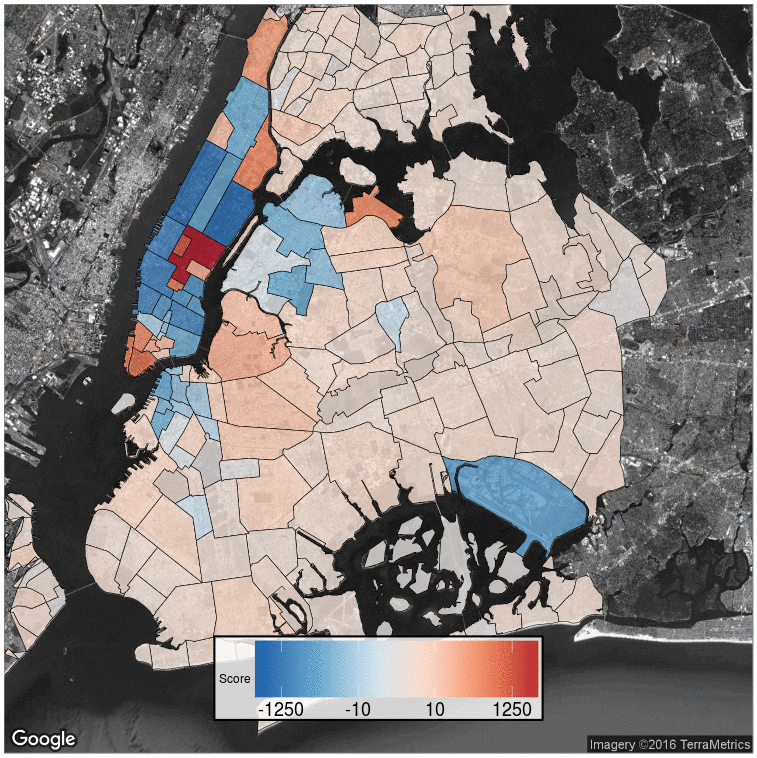
\includegraphics[width=0.24\textwidth]{7am} 
 %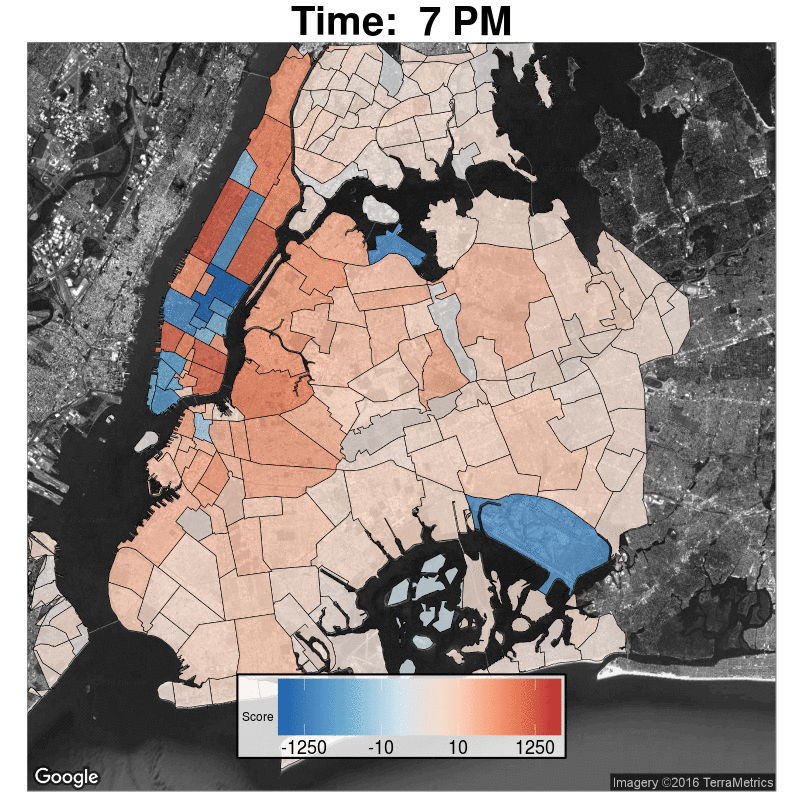
\includegraphics[width=0.24\textwidth]{7pm}
 
 % 
\begin{subfigure}{0.24\textwidth}
\centering
 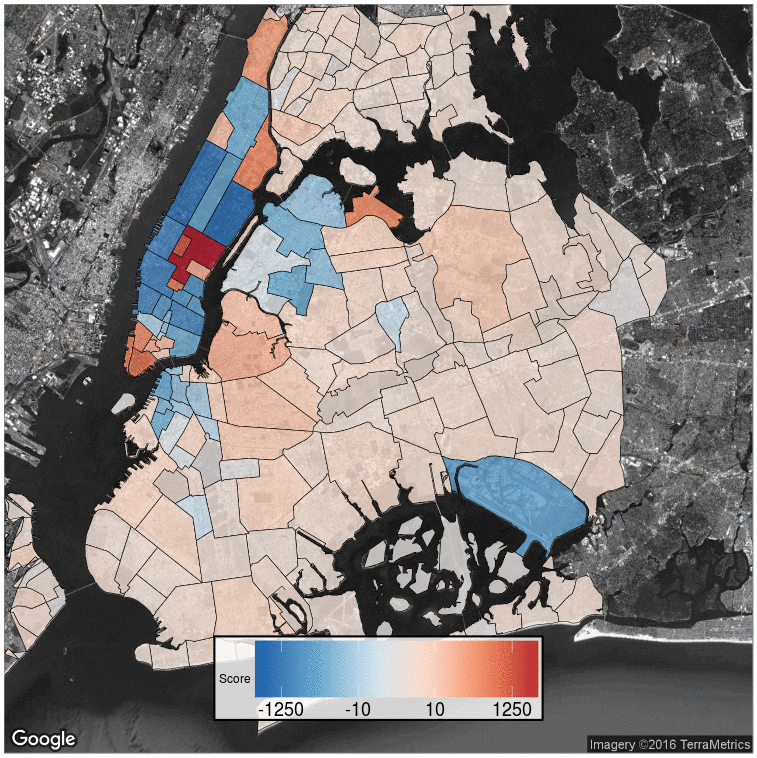
\includegraphics[width=1\linewidth]{7am} 
 \caption{7 AM}
 \label{fig:7am}
\end{subfigure}
 \begin{subfigure}{0.24\textwidth}
 \centering
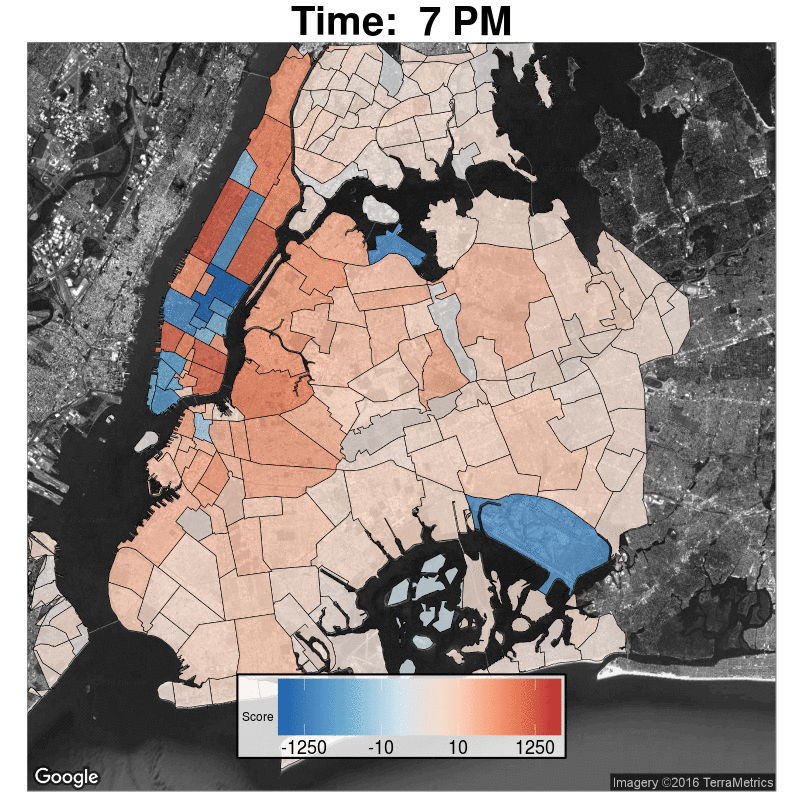
\includegraphics[width=1\linewidth]{7pm}
 \caption{7 PM} 
 \label{fig:7pm}
\end{subfigure}
 
\caption{Net Flow of people during weekdays in July '13}
\label{fig:flow}
\end{figure}

\section{Driver and Shift Efficiency}
Given this high-level understanding of how people move throughout the city, next we investigated the role of drivers in the taxi system. In particular, we looked at two questions: first, how do driver earnings vary, and second, how much of this variation is due to skill versus chance?
%By answering these questions, we can assess whether or not drivers have significantly varying skill levels.

We began by computing the efficiency of a driver in a work period, defined as the ratio of the total metered fare earned in that period to the total time worked. The total metered fare earned on each trip was available directly in our data set. Unfortunately, however, the data does not contain the time each driver spent working in a shift; rather, it only logs the times that a driver was with a passenger, making it difficult to identify the length of a shift. Previous work used the distance between a dropoff and the next pickup to approximate total shift time~\cite{LEE:2015}. We took a more refined approach to identify driver shifts by looking at the downtime, or time between a drop off and the next pickup, for all trips.
Consistent with past work on driver earnings~\cite{Farber:2014}, we found that very few drivers have downtimes of six hours, with the time between most trips either ranging from a few minutes to 12 hours. %(figure ~\ref{fig:downtime_distribution}).
Accordingly, we defined any dropoff where there is no driver activity for at least six hours as the end of a shift, with the following pickup marking the beginning of a new shift.
With this information we were able to group each driver's rides into shifts and compute driver efficiency for each shift as defined above.

%Figure~\ref{fig:downtime_distribution} shows the distribution of downtimes for all drivers. 
%Looking at this distribution, we defined the end of a shift as the last drop off when there is no driver activity for at least six hours, which agrees with previous research studying driver earnings~\cite{Farber:2014}. The next pickup marked the beginning of the next shift. With this shift information, we were able to group each driver's rides into shifts and compute the efficiency for each shift.

%\begin{figure}[t]
%  \centering
%  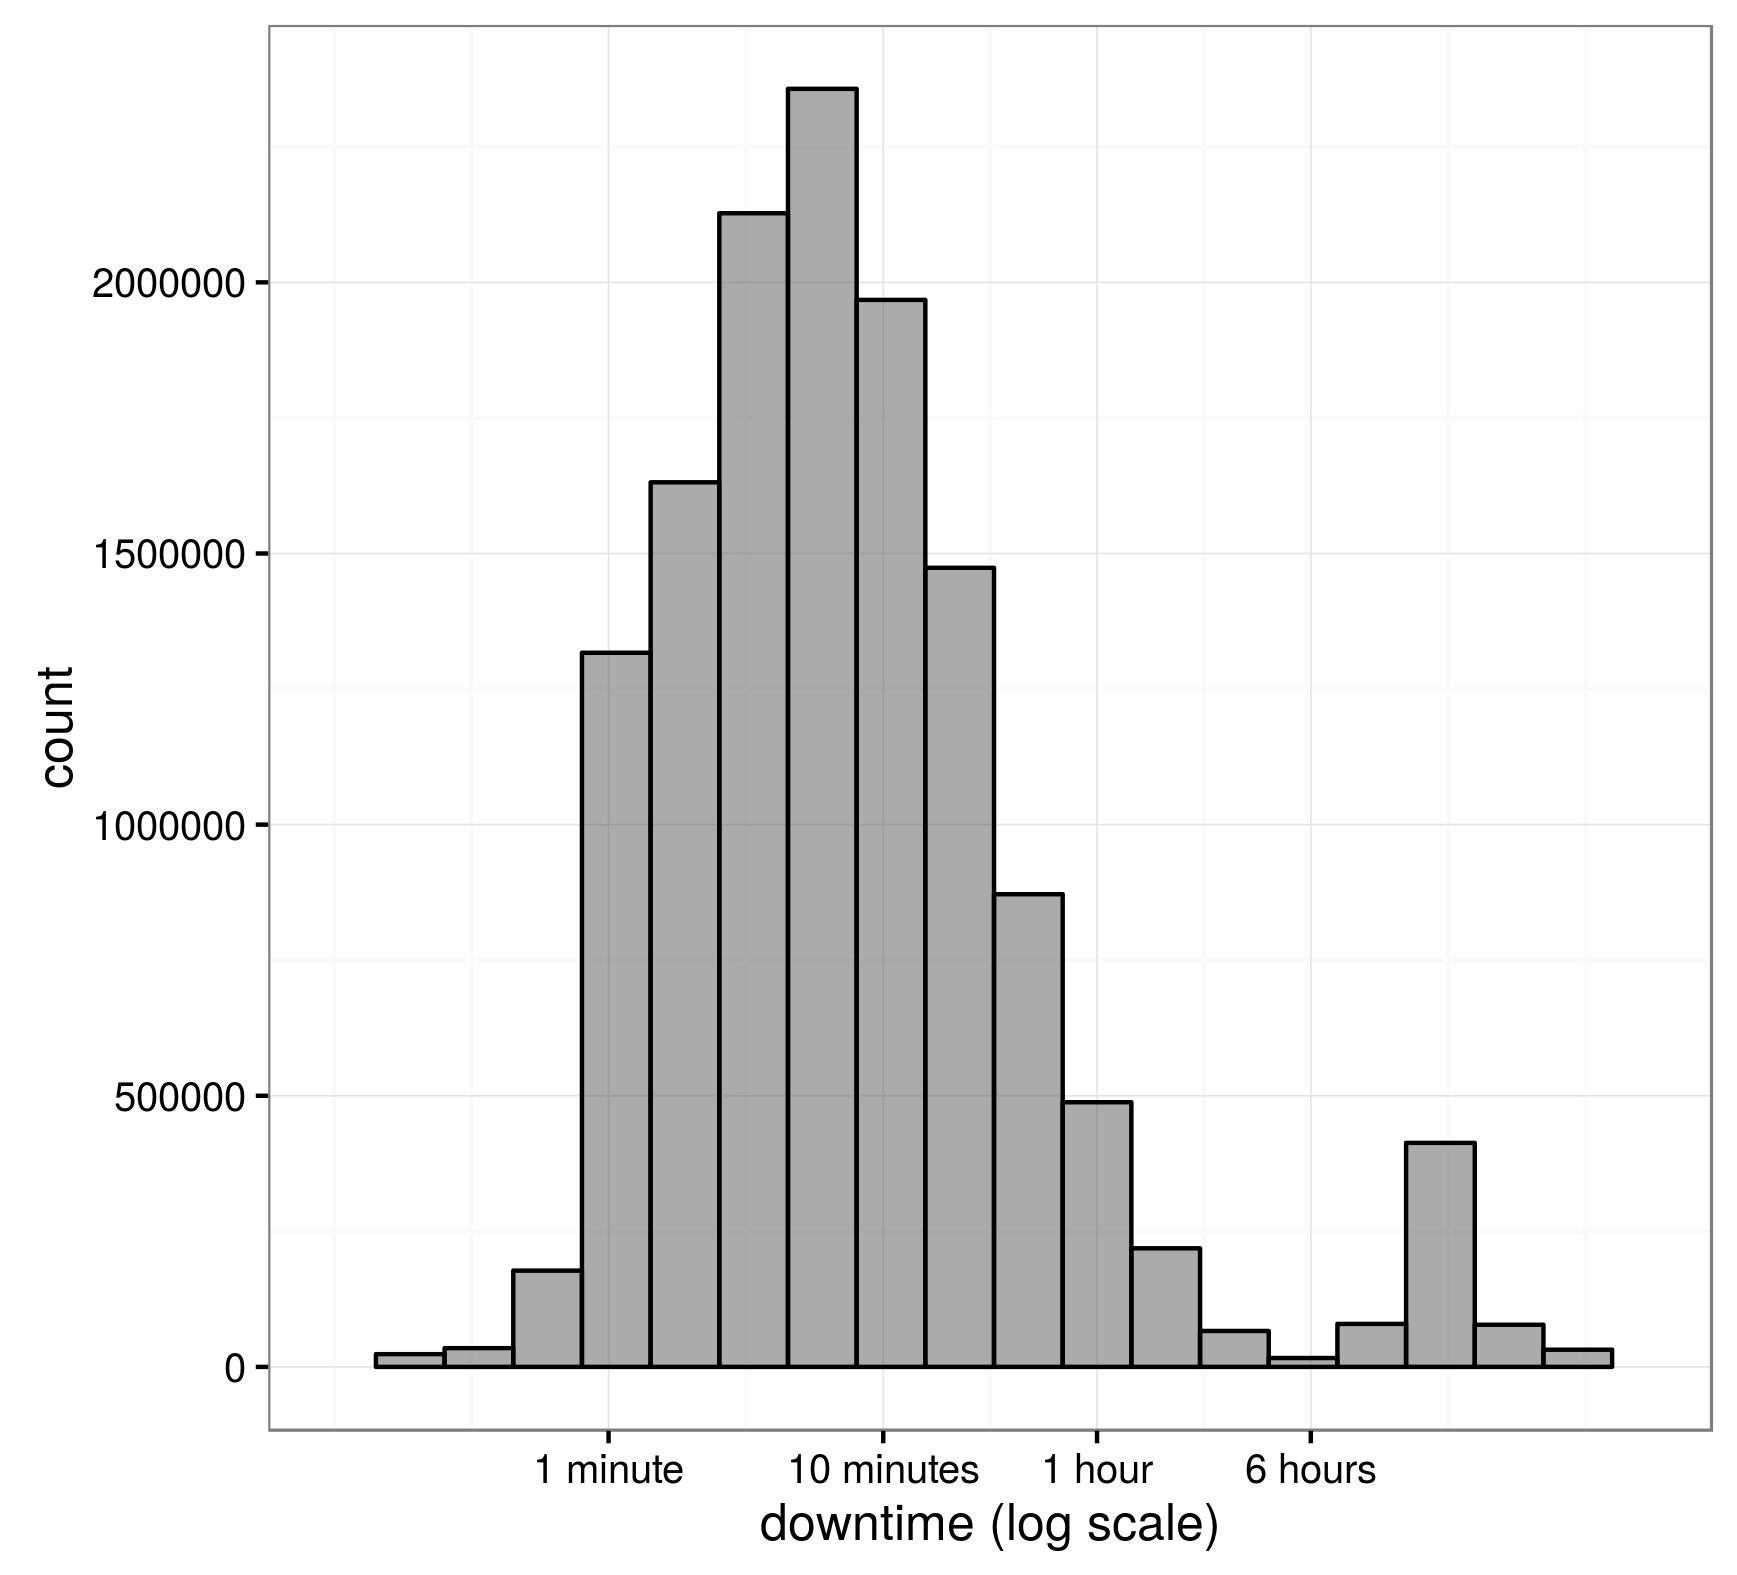
\includegraphics[width=.9\linewidth]{downtime_distribution}
%  \captionof{figure}{Downtimes for all rides. We see that there are very few drivers who have a 6-hour gap between two rides.}
%  \label{fig:downtime_distribution}
%\end{figure}
\begin{figure}[t]
  \centering
  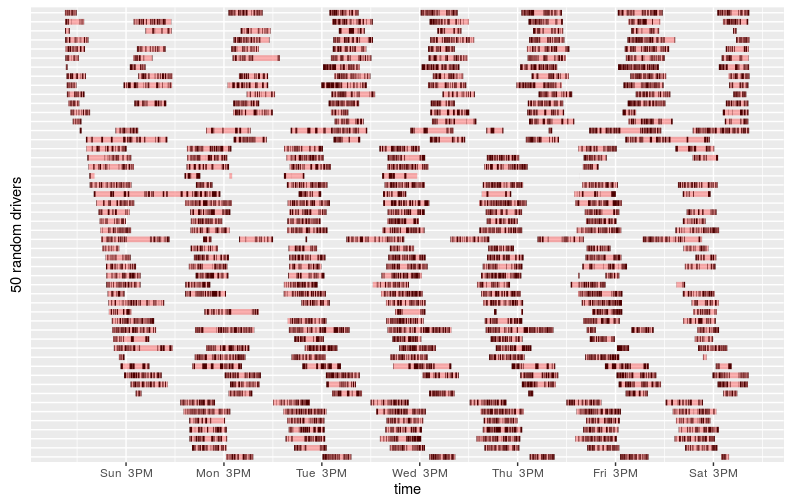
\includegraphics[width=1\linewidth]{shifts_id}
  \captionof{figure}{Rides (in black) and shifts (in red) for 50 random drivers over a week's time in July.}
  \label{fig:shifts_id}
\end{figure}
Doing so revealed that drivers have passengers for approximately half of their shift time and earn an average of \$30 per shift, with a reasonable amount of variation in earnings across drivers.
That said, it is unclear what drives this variation---is it simply due to the string of pickup and dropoff locations a driver happens to be assigned, or can it be attributed to some inherent difference in skill across drivers?
To better understand variation in efficiency, we fit a linear regression to predict shift efficiency using the following model:
%Now, we wanted to find out what effect the driver has on the efficiency of shifts. To accomplish that, we ran a linear regression, using the following model: 
\begin{eqnarray*}
&& \beta_{\mathrm{driver~id}} + \beta_{\mathrm{hour}} + \beta_{\mathrm{weekend}} + \beta_{\mathrm{hour:weekend}} + \\
  & & \gamma_p x_p + \sum_{n=1}^N \rho_n p_n + \sum_{n=1}^N \delta_n d_n,
\end{eqnarray*}
where each $\beta$ represents the effect of its corresponding subscript---whether it be the driver's ID, the start hour of a shift, or whether it is a weekend of the weekday---$x_p$ is precipitation in inches, and $\gamma_p$ is its coefficient. The two summations represent the percentage of pickups ($p_n$) and drop-offs ($d_n$), respectively, in each neighborhood, with $\rho$ and $\delta$ as their coefficients.

After running our model, we observed a significant variance in earnings, with some drivers consistently making $\pm$$\$$10/hour from the average. However, this model does not necessarily confirm the correlation between drivers and earnings, as the high variance could have been due to chance. To see what we would expect from chance, we randomized the assignment of drivers to shifts and re-ran our regression. In the randomized data set, the variance was cut in half to $\pm$$\$$5/hour (Figure~\ref{fig:efficiency}). The difference between the distributions of earnings signifies that the actual variation in driver earnings is not due to chance. There are drivers who make a great deal more than the average driver, as well as drivers who make a great deal less. Thus, while anyone can become a cab driver, there are certain skills that distinguish a driver from others. 
\begin{figure}[h]
  \centering
  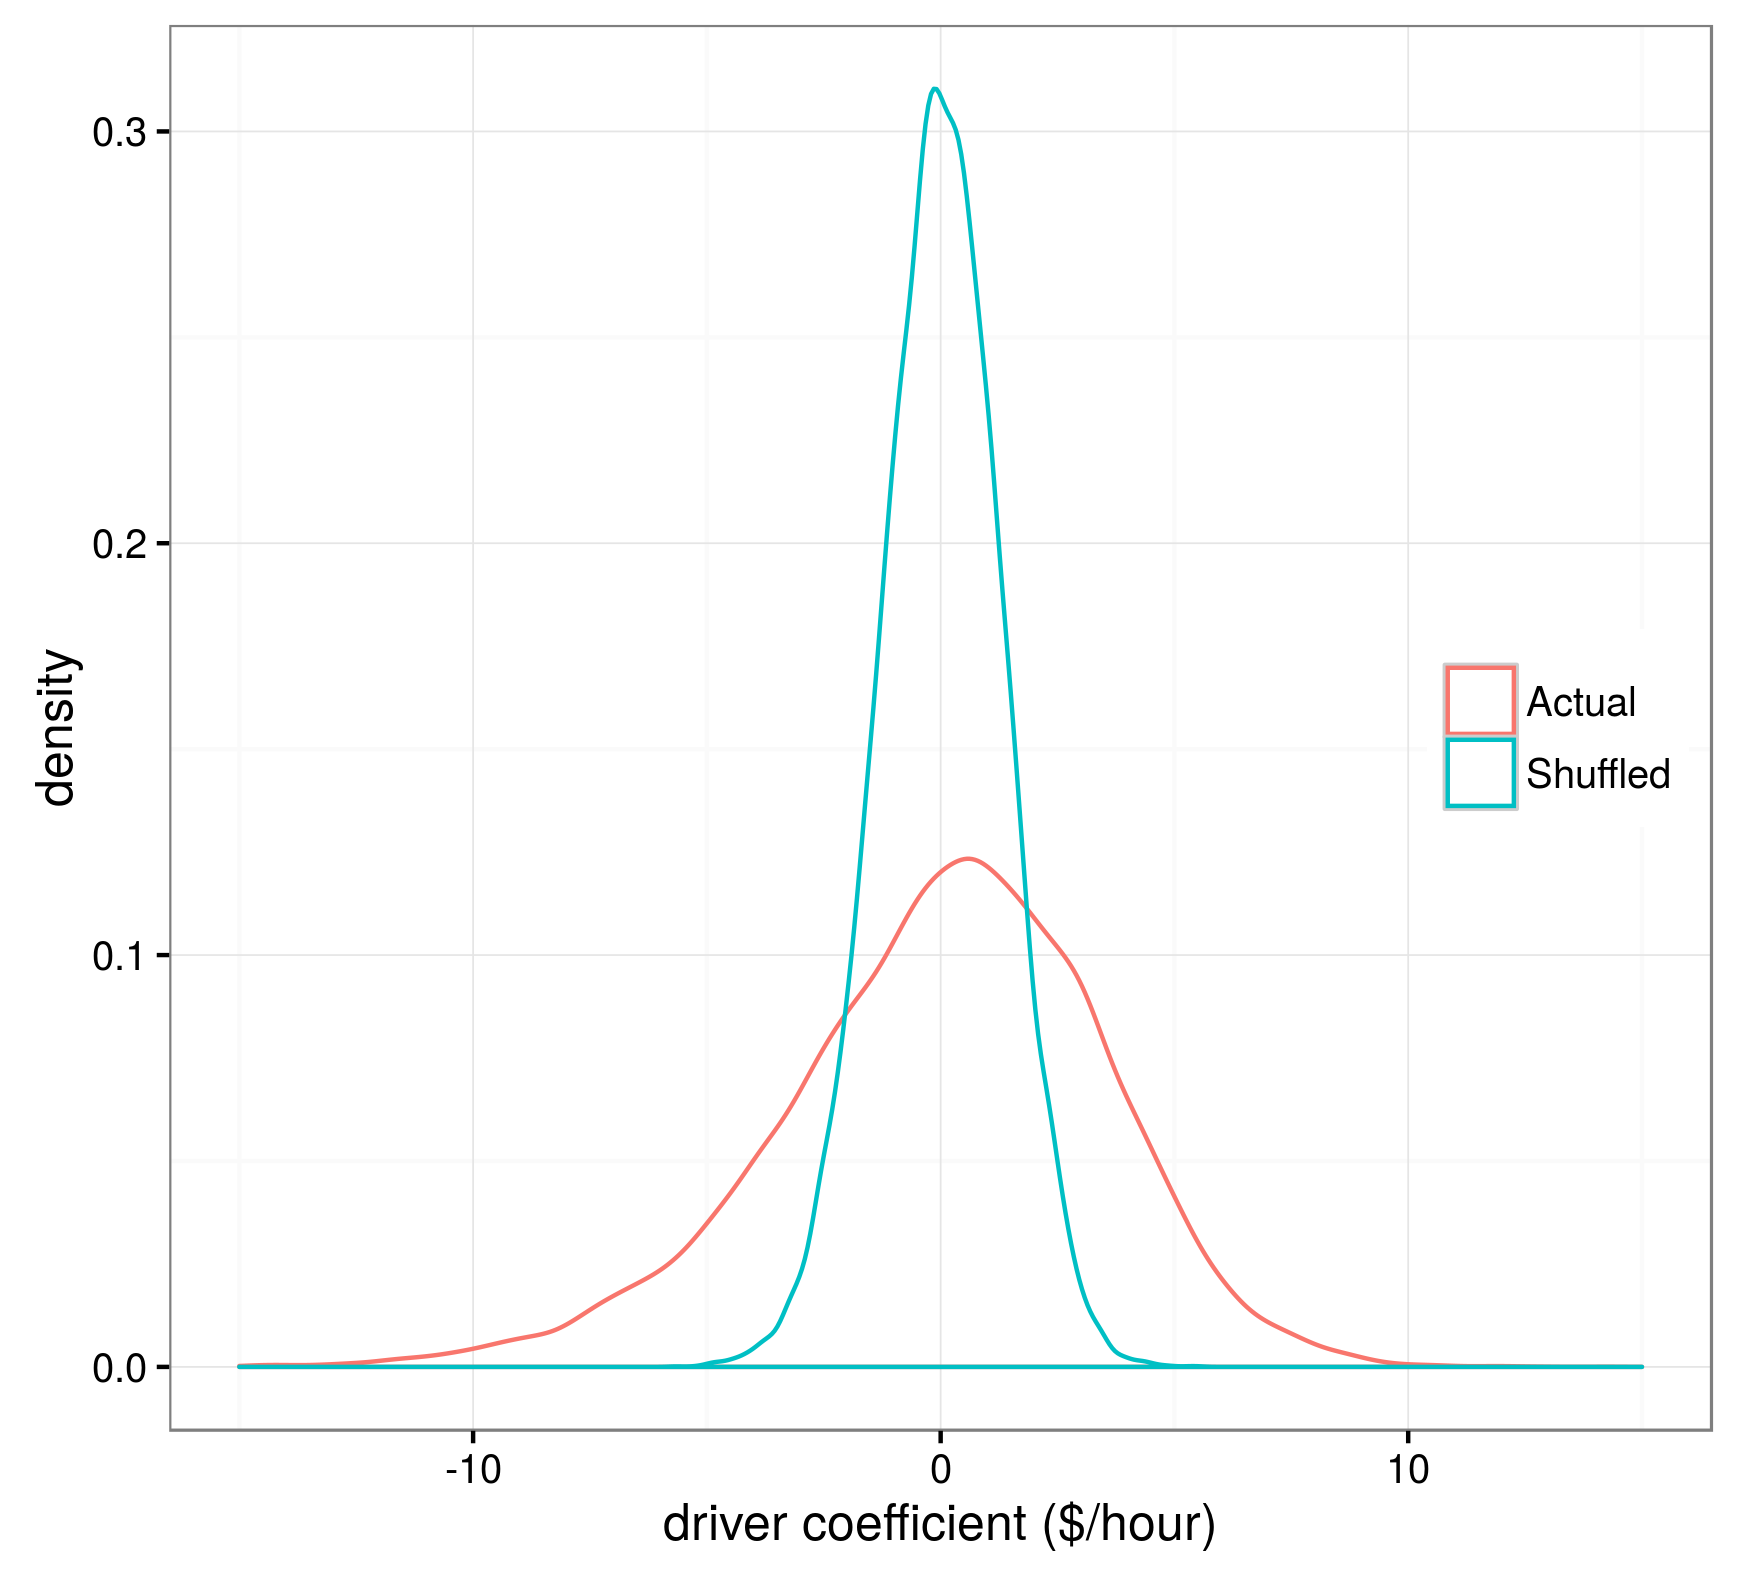
\includegraphics[width=.9\linewidth]{efficiency}
  \captionof{figure}{Effect of Driver ID on Efficiency}
  \label{fig:efficiency}
\end{figure}
\section{Carpooling}
After looking at flow and driver behavior, we wanted to find ways to improve the overall taxi system. Past work have focused on recommender systems~\cite{ZHAN:2014} or information systems~\cite{KIM:2005}, which would require taxi drivers to be notified via a mobile application or a similar solution. We take a different approach and look at a policy that can be implemented at existing taxi stands, with little overhead. We noticed that there were lots of trips occurring between similar locations. As a result, we considered a scenario in which people would carpool. Our thought experiment made the following assumptions: Customers would be willing to (1) share a cab with strangers, (2) wait up to five minutes to find someone to carpool with, (3) walk up to one block, (4) share a destination within ~1 kilometer of their own destination. We also assumed that customers would carpool only for trips between two distinct neighborhoods, because customers would probably not want to wait for trips that are relatively short.

To look for carpooling potential, we rounded the start time of trips to the nearest 5 minutes, pickup coordinates to the nearest two thousandth, and dropoff coordinates to the nearest hundredth. We then counted the number of trips and passenegers within each ``carpooling potential" bin. As we were expecting, a significant number of trips were taking place around the same location, at a similar time. After finding these trips and plotting their pick-up points on a map, we identified the top carpooling hotspots in NYC (figure~\ref{fig:hotspots}). Unsurprisingly, many of these places are either major transportation hubs (JFK airport, LaGuardia airport, Penn Station, Port Authority Bus Terminal, and Grand Central Terminal) or popular cultural attractions (the Metropolitan Museum of Art, the Lincoln Center, the Theater District, etc.). 
\begin{figure}[h]
  \centering
  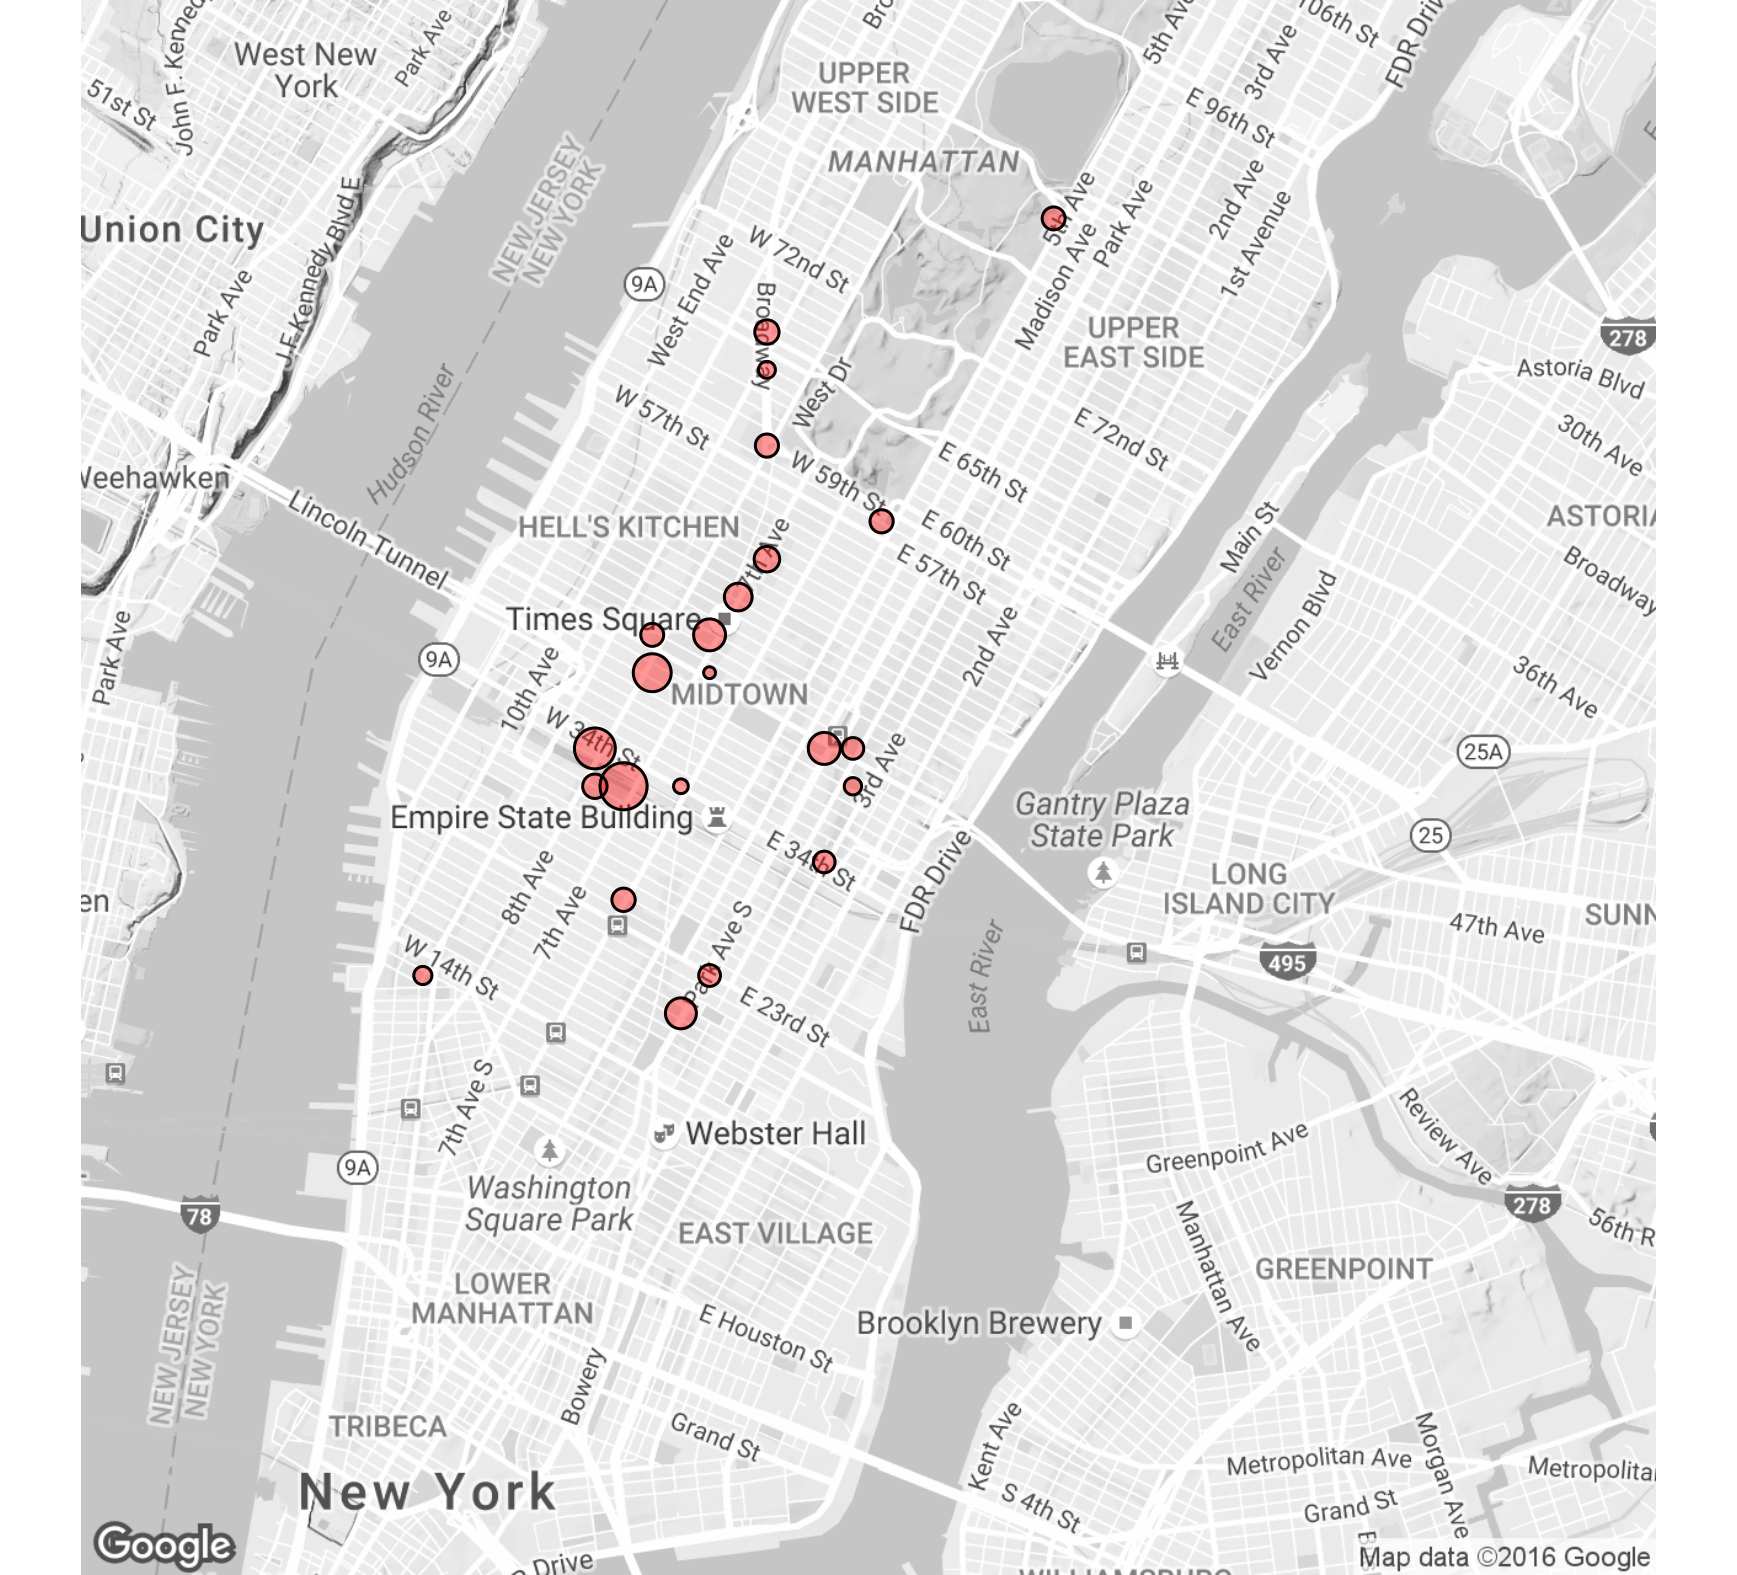
\includegraphics[width=.9\linewidth]{top_25_hotspots}
  \captionof{figure}{Top carpooling hotspots in Manhattan. Points are sized by how frequent a carpooling potential occurs at a location.}
  \label{fig:hotspots}
\end{figure}

Next, we calculated our potential savings. We assumed that up to 4 passengers would fit in one cab (since 92\% of taxis fit 4 passengers~\cite{TLC:2007}). The minimum number of trips needed per each 5 minute bin is given by $\ceil{\mathrm{number~of~passengers}\div4}$. The number of ``unecessary" trips per bin are thus $\mathrm{actual~number~of~trips} - \mathrm{minimum~number~of~trips~needed}$, and the potential fare savings are $\mathrm{average~fare~per~trip}\times\mathrm{``unnecessary"~trips}$. Our potential savings over the month of July were over 650,000 thousands trips, around 5\% of total trips and over 8.5 million dollars, around 6\% of total money spent by customers.

We also found that with less restrictive assumptions, i.e. widening the waiting period to 6 minutes, and including rides taking place within the same neighborhood, we can improve the savings up to 14\% for the number of rides and fare paid. In addition to saving money, carpooling would also help the environment and reduce traffic! 

\section{Acknowledgements}
We thank our mentors Ashton Anderson (Microsoft Research), Christopher Riederer (Columbia University), Jake Hofman (Microsoft Research), and Siddhartha Sen (Microsoft Research) for their mentorship as a part of the 2016 Microsoft Research Data Science Summer School. Maps were produced using the ggmap package in R~\cite{KAHLE:2013}.

% Bibliography
%\vspace{-0.5em}
\bibliographystyle{unsrt}
\bibliography{refs}
\end{document}
%%% Local Variables:
%%% mode: latex
%%% TeX-master: t
%%% End:
\grid
